
\element{general}{
  \begin{question}{prez}
    Among the following persons, which one has ever been a President of the French Republic?
    \begin{choices}
      \correctchoice{Rene Coty}
      \wrongchoice{Alain Prost}
      \wrongchoice{Marcel Proust}
      \wrongchoice{Claude Monet}
    \end{choices}
  \end{question}
}

\element{general}{
  \begin{questionmult}{pref}
    Among the following cities, which ones are French prefectures?
    \begin{choices}
      \correctchoice{Poitiers}
      \wrongchoice{Sainte-Menehould}
      \correctchoice{Avignon}
    \end{choices}
  \end{questionmult}
}

\element{general}{
  \begin{question}{nb-ue}
    How many different states were members of the European Union in Jan. 2009?
    \begin{choiceshoriz}[o]
      \wrongchoice{15}
      \wrongchoice{21}
      \wrongchoice{25}
      \correctchoice{27}
      \wrongchoice{31}
    \end{choiceshoriz}
  \end{question}
}




\element{mcq2}{
  \begin{question}{nb-ue}
    How many different states were members of the European Union in Jan. 2009?
    \begin{choiceshoriz}[o]
      \wrongchoice{15}
      \wrongchoice{21}
      \wrongchoice{25}
      \correctchoice{27}
      \wrongchoice{31}
    \end{choiceshoriz}
  \end{question}
}

 

\element{mcq}{
  \begin{questionmultx}{q41}\scoring{e=-1,v=0,b=4,m=-1}     
Let $G=(V,E)$ be a graph such that $\left \vert V \right \vert =7$ and $\left \vert E \right \vert =16$. Which of the following statements are true?

  \begin{multicols}{2}
    \begin{choices}
      \correctchoice{$G$ connected.}
      \wrongchoice{$G$ is planar.}
      \wrongchoice{$G$ is Eulerian}
      \wrongchoice{$G$ has a perfect matching.}
    \end{choices}
   \end{multicols}

  \end{questionmultx}
}


\element{mcq}{
  \begin{questionmultx}{44}\scoring{e=-1,v=0,b=4,m=-1}     
Which of the graphs given below are planar?
\begin{center}
  
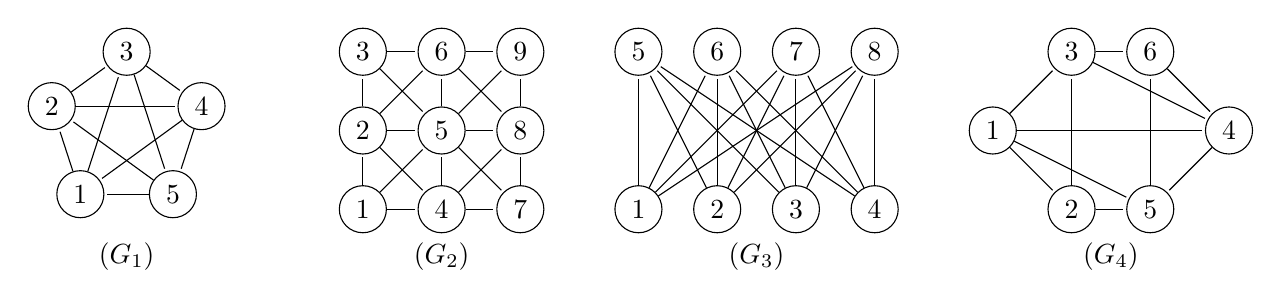
\begin{tikzpicture}[shorten >=1pt]
  \tikzstyle{vertex}=[circle,draw,minimum size=17pt,inner sep=0pt]
  \foreach \name/\angle/\text in {P-1/234/1, P-2/162/2, P-3/90/3, P-4/18/4, P-5/-54/5}
    \node[vertex,yshift=.5cm] (\name) at (\angle:1cm) {$\text$};
  \foreach \from/\to in {1/2,2/3,3/4,4/5,5/1,1/3,2/4,3/5,4/1,5/2}
    { \draw (P-\from) -- (P-\to); }

    \foreach \i/\j/\text in {1/1/1,1/2/2,1/3/3,2/1/4,2/2/5,2/3/6,3/1/7,3/2/8,3/3/9}
      \node[vertex,xshift=2cm,yshift=-1.5cm] (Q-\text) at (\i,\j) {$\text$};
     \foreach \from/\to in {1/2,1/4,1/5,2/4,2/5,4/5,2/3,2/6,3/5,3/6,5/6,6/8,6/9,8/9,5/7,5/8,5/9,4/8,4/7,7/8}
    { \draw (Q-\from) -- (Q-\to); }
 
 \foreach \i/\j/\text in {1/1/1,1/2/2,1/3/3,1/4/4, 3/1/5,3/2/6,3/3/7,3/4/8}
      \node[vertex,xshift=5.5cm,yshift=-1.5cm] (R-\text) at (\j,\i) {$\text$};
     \foreach \from/\to in {1/5,1/6,1/7,1/8,2/5,2/6,2/7,2/8,3/5,3/6,3/7,3/8,4/5,4/6,4/7,4/8}
    { \draw (R-\from) -- (R-\to); }

 \foreach \i/\j/\text in {1/2/1,2/1/2,2/3/3,4/2/4, 3/1/5,3/3/6}
      \node[vertex,xshift=10cm,yshift=-1.5cm] (S-\text) at (\i,\j) {$\text$};
     \foreach \from/\to in {1/2,1/3,2/3,4/5,5/6,6/4,1/4,2/5,3/6,3/4,1/5}
    { \draw (S-\from) -- (S-\to); }

 \foreach \i/\text in {0/1,4/2,8/3,12.5/4}
      \node[yshift=-1.1cm] (T-\text) at (\i,0) {$(G_{\text})$};
 

\end{tikzpicture}

\end{center}

  \begin{multicols}{3}
    \begin{choices}
      \wrongchoice{$G_{1}$}
      \correctchoice{$G_{2}$}
      \wrongchoice{$G_{3}$}
      \correctchoice{$G_{4}$}
    \end{choices}
     \end{multicols}

  \end{questionmultx}
}




\element{mcq}{
  \begin{questionmultx}{45}\scoring{e=-1,v=0,b=4,m=-1}     
Consider the graph $G$ given below. The numbers on each edge denotes the {\it weight} of the corresponding edge.The weight of an edge $e$ is denoted by $w(e)$. The {\it weight of a graph} is defined to be $\sum_{e \in E}w(e)$. Let $T$ be a least weighted connected subgraph of $G$ containing $9$ vertices.  Which of the following statements are true?




\begin{center}
\scalebox{.6}{
\begin{tikzpicture}[-,>=stealth',shorten >=1pt,auto,node distance=2.5cm,
                    semithick]
  \tikzstyle{every state}=[draw,text=black,minimum size=12pt,inner sep=0pt]

  \node[state]         (A)              			{$A$};
  \node[state]         (B) [right of=A,above of=A] 		{$B$};
  \node[state]         (C) [right of=B] 			{$C$};
  \node[state]         (D) [below of=A] 			{$D$};
  \node[state]         (E) [below of=B,yshift=7mm]		{$E$};
  \node[state]         (F) [below of=C,yshift=7mm] 		{$F$};
  \node[state]         (G) [right of=D,yshift=15mm]		{$G$};
  \node[state]         (H) [below of=C,yshift=-1cm]		{$H$};
  \node[state]         (I) [below of=H,right of=H,yshift=1cm] 	{$I$};

\path (A) edge node[xshift=01mm]			 { 1}(B);
\path (B) edge node[xshift=01mm]			 { 2}(C);
\path (A) edge node[xshift=01mm]			 { 3}(E);
\path (B) edge node[xshift=-1mm]			 { 4}(E);
\path (D) edge node[xshift=01mm]			 { 5}(A);
\path (C) edge node[xshift=-1mm]			 { 6}(F);
\path (E) edge node[xshift=01mm]			 { 7}(C);
\path (E) edge node[xshift=01mm]			 { 8}(F);
\path (D) edge node[xshift=01mm]			 { 9}(E);
\path (C) edge node[xshift=-2mm]			 {10}(I);
\path (I) edge node[yshift=02mm]			 {11}(F);
\path (D) edge node[xshift=03mm]			 {12}(H);
\path (I) edge node[xshift=01mm]			 {13}(H);
\path (D) edge node[xshift=01mm]			 {14}(I);
\path (H) edge node[xshift=00mm]			 {15}(F);
\path (G) edge node[xshift=01mm]			 {16}(E);
\path (G) edge node[xshift=01mm]			 {17}(H);
\path (D) edge node[xshift=03mm]			 {18}(G);
                                                          
\end{tikzpicture}}
\end{center}


  \begin{multicols}{2}
    \begin{choices}
      \correctchoice{$T$ contains exactly $8$ edges}
      \correctchoice{$T$ doesn't contain the edge $(G,D)$}
      \correctchoice{$T$ does contain the edge $(A,B)$}
      \wrongchoice{$T$ is not bipartite.}
    \end{choices}
    \end{multicols}

  \end{questionmultx}
}


